\chapter{Track Reconstruction}
\label{sec:track}
	The~first stage of our reconstruction algorithm is the~reconstruction of the track of the~primary particle (electron or positron). The~results of this step are then used to determine the~energy of the~particle (see section~\ref{sec:energy}).
	
	\textbf{First Attempts} at a~track reconstruction were made using the~standard approach. Here we assume we know the~readout coordinates ($x'$,~$y'$,~$t$) exactly (i.e. we neglect the~pads and time bins). In standard \ac{TPC} (with parallel fields) we only need to reconstruct the~$z$~coordinate from drift time using the~known drift velocity.
	
	Reconstruction with the~\textbf{Ionization Electron Map} (from now on referred to as \emph{the~map}) uses simulation of the~drift of the~secondary (ionization) electrons in the~volume of the detector. This simulation can then be used to interpolate the~initial position of the~secondary electrons. First attempts neglect the~pads.
	
	The~\textbf{Discrete Reconstruction} is made using the~map, instead of reconstructing the~exact position of each electron we reconstruct the middle point of each hit pad with time corresponding to the~middle of the~time bin. The number of electrons in each \ac{TPC}~bin (consisting of the~pad and the~time bin) is counted and used as a~charge in the~energy reconstruction.
	
	\textcolor{red}{Reconstruction of one track simulated with microscopic tracking in Garfield++.}
	
	\section{First Attempts}
	\label{sec:trackfirst}
		As the~first step of the~work, we decided to try to reconstruct an~electron track with a~special set of initial parameters. The~origin of the~particle is given by the~origin of our coordinate system. The initial direction is given by the~positive $x$~axis. This means the~magnetic field of our detector is perpendicular to the~momentum of our particle at all times and we can reduce the problem to two dimensional space. We use a~track simulated using the~microscopic simulation (see section~\ref{sec:microsim}) with a~kinetic energy of 8~MeV. The gas composition used in this simulation is 90\%~Ar~+~10\%~CO$_2$.
		
		In this first approach to the~reconstruction of the~track, we decided to use the~common method used in a~standard \ac{TPC}. This will allow us to explore the significance of the~atypical behavior in our \ac{OFTPC}. At the~same time, we consider the~readout to be continuous to further simplify the~problem. In this approximation we reconstruct the~initial position of each ionization electron.
		
		The~reconstruction is then defined by the~following relations between the~coordinates of the~detector space and the~readout space (see section~\ref{sec:coor}):
			\begin{eqnarray}
				x = x',\\
				y = y',\\
				z = v_d t,
			\end{eqnarray}
		where $v_d$ is the~drift velocity of electrons in the~given gas mixture. On a~phenomenological level, this velocity can be considered a~function of the~electric field~$\bm{E}$ and the~magnetic field~$\bm{B}$:
			\begin{equation}
				v_d = v_d(\bm{E},\bm{B}).
			\end{equation}
		\textcolor{red}{Taken from Garfield user manual.} The~Garfield++ toolkit uses this fact to accelerate their drift simulation with non-microscopic approaches. Since we assume uniform electric field in our detector and we want to neglect the~effect of our unusual magnetic field, we consider the~drift velocity to be constant in this scenario. We then approximate this velocity by fitting the dependence $z(t)$ taken from the~simulated ionization electrons.\textcolor{red}{This is in one of the provisional figures. Also this description is not completely accurate, in reality we fit t1:8-y0 with a1*x+a0 and then invert this and use 8-y0 = b1*t1+b0 (old coordinates), b1=1/a1 functions as the drift velocity. Maybe also define this 8-z variable as an alternative to z in the section~\ref{sec:coor} and then use it when correcting this.}
		
		\textcolor{red}{Later, in a commit after this, I plot some residues (provisional figure) which could be useful but for some reason they are residuals from a spline fit of the track?! Probably redo this without the spline fit, just explore the difference in individual points.}
		
		\begin{figure}
			\centering
			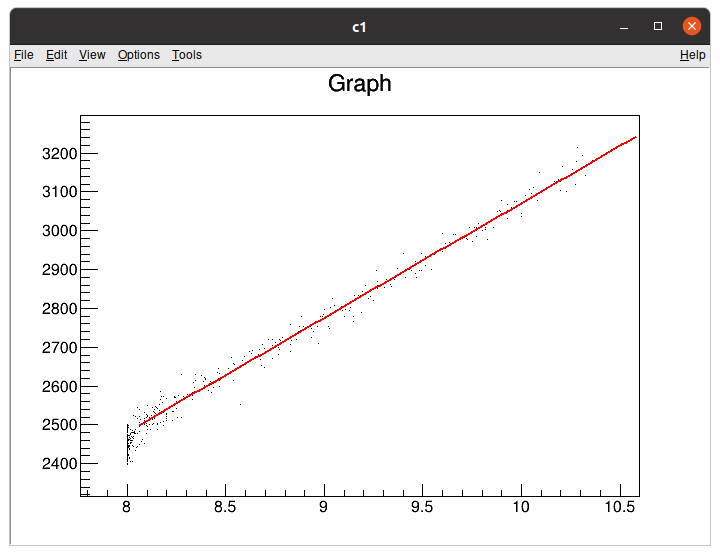
\includegraphics[width=0.5\textwidth]{9010_zt.png}
			\caption{Dependence of the~drift time on the~$z$~coordinate in 90~\%~argon and 10~\%~CO$_2$ atmosphere, fitted with a~linear function. The~fitted function gives us the~average drift velocity in the~gas and can be used for rough reconstruction in our \ac{TPC}. \textcolor{red}{Swap for better image with axis labels, etc. Maybe write the~fitted equation.}}
			\label{fig:9010zt}
		\end{figure}
		
		\begin{figure}
			\centering
			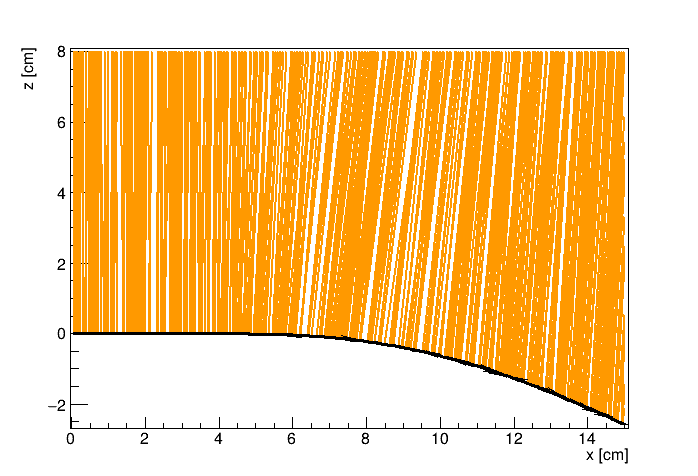
\includegraphics[width=0.5\textwidth]{9010_xz.png}
			\caption{First attempt at a~track reconstruction using only the~drift velocity. This approach works well in a~standard \ac{TPC} (\textcolor{red}{ideally cite some source?}). 90~\%~argon and 10~\%~CO$_2$ atmosphere. \textcolor{red}{Swap for better image, correct coordinates.}}
			\label{fig:9010xz}
		\end{figure}
		
		\begin{figure}
			\centering
			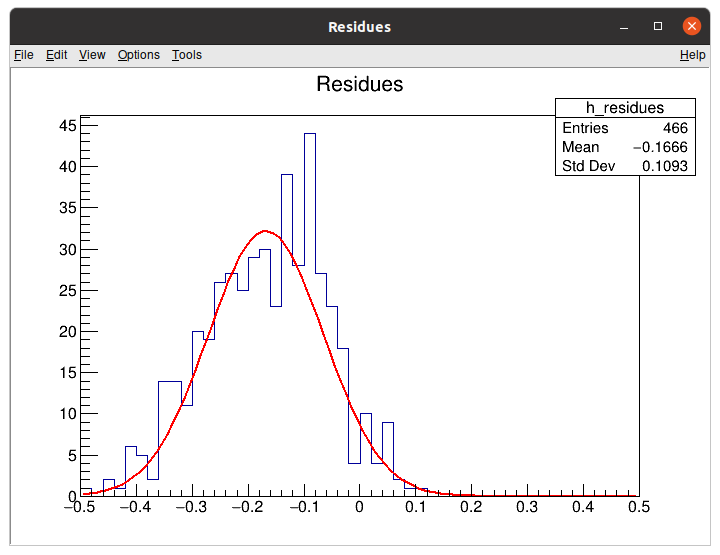
\includegraphics[width=0.5\textwidth]{9010_res.png}
			\caption{First attempt at a~track reconstruction using only the~drift velocity, residues. \textcolor{red}{Swap for better image, correct coordinates. What's causing the shift? Explain details.}}
			\label{fig:9010res}
		\end{figure}
	
	\section{Ionization Electron Map}
	\label{sec:map}
		For a~trajectory inside an~\ac{OFTPC}, the~drift of the~secondary (ionization) electrons is significantly affected by its magnetic field. We need to take this into account for accurate reconstruction. In the~first approximation, we assume a~continuous read out (i.e. we neglect pads). We can then reconstruct the~original position of each ionization electron using its readout coordinates. For this purpose, we use the~ionization electron map.
		
		The~ionization electron map is a~mapping between the~detector space and the~readout space. It tells us what readout coordinates $(x',y',t)$ we can expect on average for an~ionization electron created in the~detector coordinates $(x,y,z)$. To get an~approximation of this mapping, we can simulate the~drift of ionization electrons created on a~regular grid inside the~volume of our \ac{OFTPC}. It is also useful to simulate multiple (100 in our case) electrons originating in the same position so we can get a~better approximation of the~average drift. In order to get accurate results, we use the~microscopic simulation of these electrons described in the~section~\ref{sec:microsim}.
		
		Finally, we need to invert the~map to get the~original detector coordinates $(x,y,z)$ for given readout coordinates $(x',y',t)$. \textcolor{red}{Two ways of inverting.}
		
		The~simulation of the~map is a~computationally heavy task. For this reason, we use a~grid MetaCentrum \textcolor{red}{(citation)} to parallelize it. At first, this was done by splitting the~simulated electrons evenly between the~individual jobs. This was used in the~first simulation with only one electron per vertex in the~regular grid with the~spacing of one centimeter. 
		
		Later a~better approach was used accounting for different lengths of the~trajectory of individual electrons. If we index the~electrons in the~order of increasing coordinates $y,x,z$ (\textcolor{red}{picture?}), we can express the~number~$n_l$ of full XY~layers (electrons with the~same $z$~coordinate) of electrons with index less than or equal to $i$
			\begin{equation}
				n_l(i) = \left\lfloor\frac{i}{n_{xy}}\right\rfloor,
			\end{equation}
		where $n_{xy}$ is the~number of electrons in each XY~layer calculated simply by counting the~electrons that satisfy boundary conditions for $x$~and~$y$. \textcolor{red}{These conditions should be mentioned above, sector condition + maximal $x$ value.} The~number of electrons remaining in the~top layer is then
			\begin{equation}
				n_r(i) = i\!\!\!\!\mod n_{xy}.
			\end{equation}
		Finally, we can calculate the sum of the~drift gaps of electrons up to index~$i$
			\begin{equation}
				d_\text{sum} = (z_\text{max}-z_\text{min})n_{xy}n_l-\frac{n_l(n_l-1)}{2}n_{xy}l+n_r(z_\text{max}-z_\text{min}-n_l l).
			\end{equation}
		We then use the~binary search algorithm to look for the~highest value of $i$ that gives us smaller value of this sum than the~fraction $\frac{\text{job id}}{\text{max job id}}$ of the total sum. This way we obtain the~minimal and the~maximal index of electrons simulated in the~given job.
		\textcolor{red}{The spacing $l$ should be probably defined above + picture of the simulating grid (1 layer). zmin zmax also}
		
		\textcolor{red}{Could insert a table here describing all 4 simulations of the map (gas composition, spacing, etc.). Simulation inside one sector (at first double angle). Extra space on sensor. Edge cases not taken into account (TPC wall). Using qsub (not sure if important).}
		
		\textcolor{red}{Explanation of the map, pictures. Simulated on MetaCentrum, workload distribution between multiple jobs. More electrons at one location to get statistics. Two methods of reconstruction using this map. Comparison of 90/10 and 70/30 maps.}
		
		\begin{figure}
			\centering
			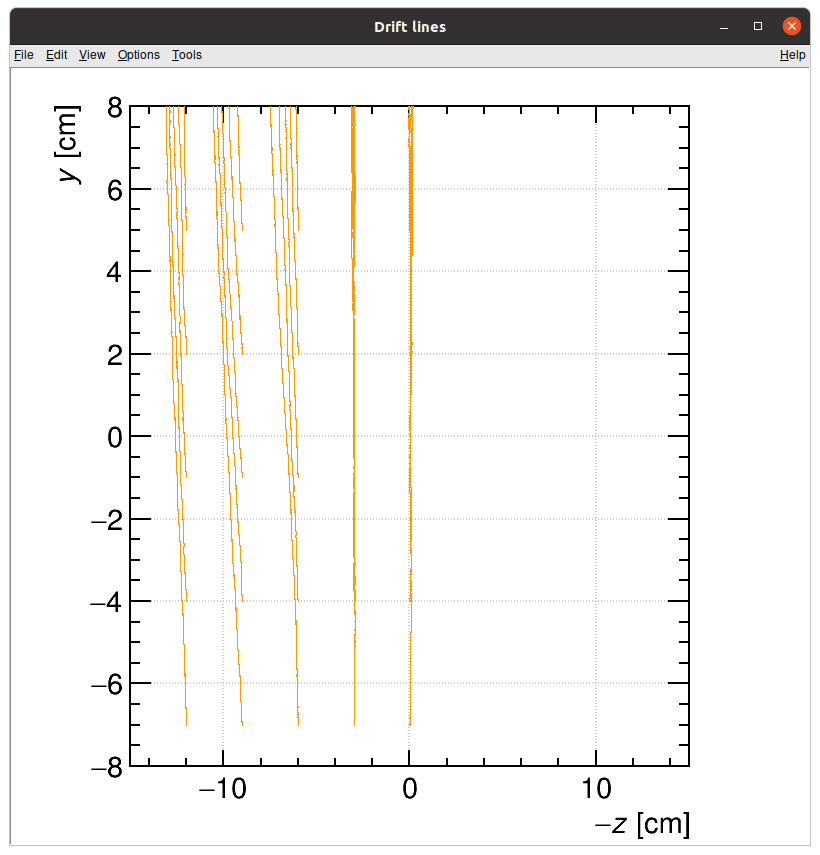
\includegraphics[width=0.5\textwidth]{map_9010_gen.png}
			\caption{Example of map generation. \textcolor{red}{Swap for better image, correct coordinates.}}
			\label{fig:map9010gen}
		\end{figure}
		
		\begin{figure}
			\centering
			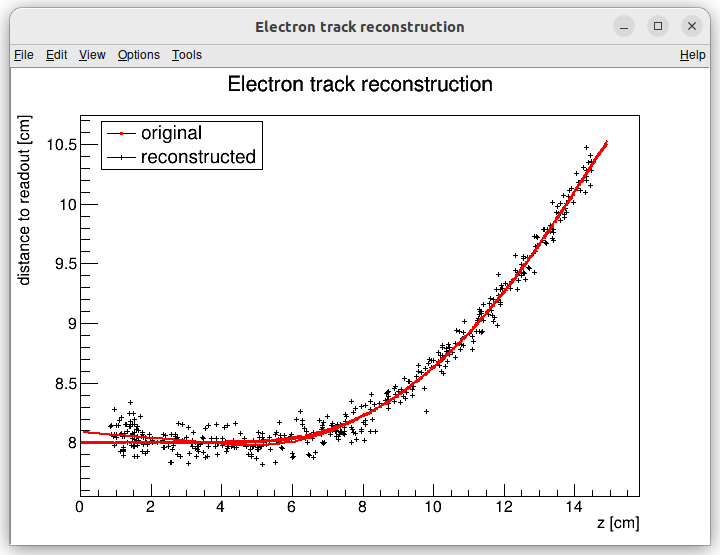
\includegraphics[width=0.5\textwidth]{9010_reco.png}
			\caption{Example reconstruction with the map. \textcolor{red}{Swap for better image, correct coordinates.}}
			\label{fig:9010reco}
		\end{figure}
		
		\subsection{Gradient Descent Search}
			\label{sec:grad}
			\textcolor{red}{Gradient descent search of a point in the original space that gets mapped to the given point of the readout space (trilinear interpolation).}
		
		\subsection{Interpolating in the Inverse Grid}
			\textcolor{red}{Interpolating between known points in the readout space. Gaussian elimination, multivariate polynomial.}
			
			\begin{figure}
				\centering
				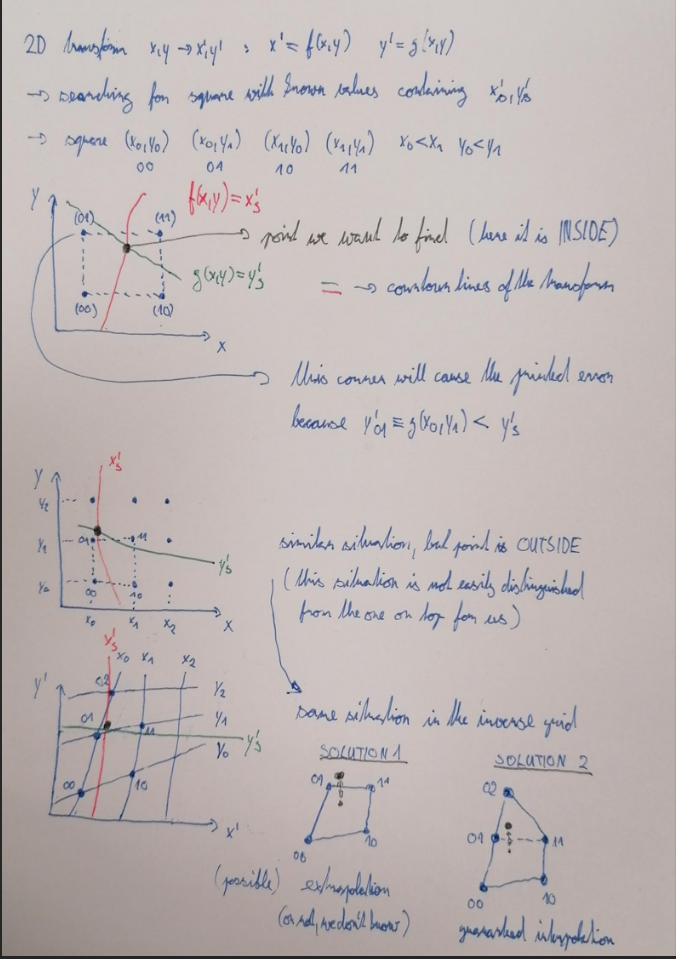
\includegraphics[width=0.8\textwidth]{interpol.png}
				\caption{Selection of the points for interpolation. \textcolor{red}{Create better images, use the explanation interpolation vs extrapolation strange property. Solution~2 probably does not make much sense.}}
				\label{fig:interpol}
			\end{figure}
		
	\section{Discrete Reconstruction}
		\textcolor{red}{Reconstruction with pads and time bins. Maybe testing different pads.}